% Fig 3.8 — CSQE (Corpus-Steered Query2Doc) pipeline
\documentclass[border=4pt]{standalone}
\usepackage{tikz}
\usetikzlibrary{positioning, arrows.meta, calc, shapes.geometric, fit, backgrounds}
\begin{document}
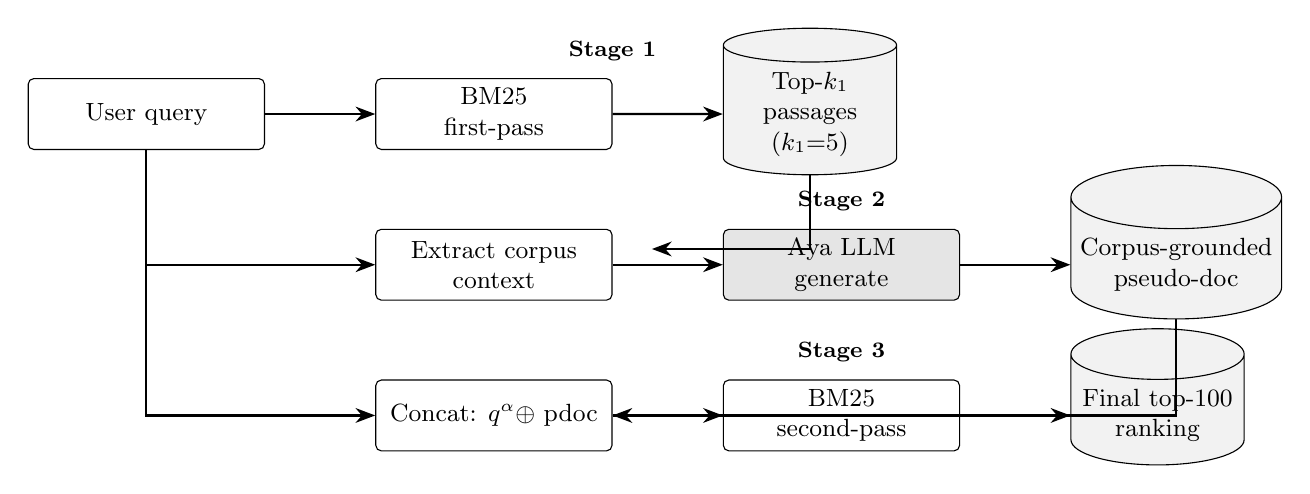
\begin{tikzpicture}[
    >=Stealth, node distance=10mm and 14mm,
    box/.style={rectangle, draw, rounded corners=2pt,
                minimum width=30mm, minimum height=9mm,
                align=center, font=\small},
    llm/.style={box, fill=black!10},
    data/.style={cylinder, shape border rotate=90, aspect=0.3, draw,
                 minimum width=22mm, minimum height=9mm, align=center,
                 font=\small, fill=black!5},
    stage/.style={font=\bfseries\footnotesize},
    arrow/.style={-{Stealth[length=2.5mm]}, thick}
]
  \node[box] (q) {User query};

  % Stage 1: first-pass retrieval
  \node[box, right=of q] (bm1) {BM25\\first-pass};
  \node[data, right=of bm1] (k5) {Top-$k_1$\\passages\\($k_1{=}5$)};

  % Stage 2: corpus context + blind generation
  \node[box, below=of bm1] (extract) {Extract corpus\\context};
  \node[llm, right=of extract] (gen) {Aya LLM\\generate};
  \node[data, right=of gen] (pdoc) {Corpus-grounded\\pseudo-doc};

  % Stage 3: second-pass with BM25 final
  \node[box, below=of extract] (concat) {Concat: $q^{\alpha} \oplus$ pdoc};
  \node[box, right=of concat] (bm2) {BM25\\second-pass};
  \node[data, right=of bm2] (final) {Final top-100\\ranking};

  \draw[arrow] (q) -- (bm1);
  \draw[arrow] (bm1) -- (k5);
  \draw[arrow] (k5.south) |- ($(extract.east) + (5mm,2mm)$);
  \draw[arrow] (q.south) |- (extract.west);
  \draw[arrow] (extract) -- (gen);
  \draw[arrow] (gen) -- (pdoc);
  \draw[arrow] (pdoc.south) |- (concat.east);
  \draw[arrow] (q.south) |- (concat.west);
  \draw[arrow] (concat) -- (bm2);
  \draw[arrow] (bm2) -- (final);

  \begin{scope}[on background layer]
    \node[stage, above=1mm of bm1.north east] {Stage 1};
    \node[stage, above=1mm of gen.north] {Stage 2};
    \node[stage, above=1mm of bm2.north] {Stage 3};
  \end{scope}
\end{tikzpicture}
\end{document}
